56. \begin{figure}[ht!]
\center{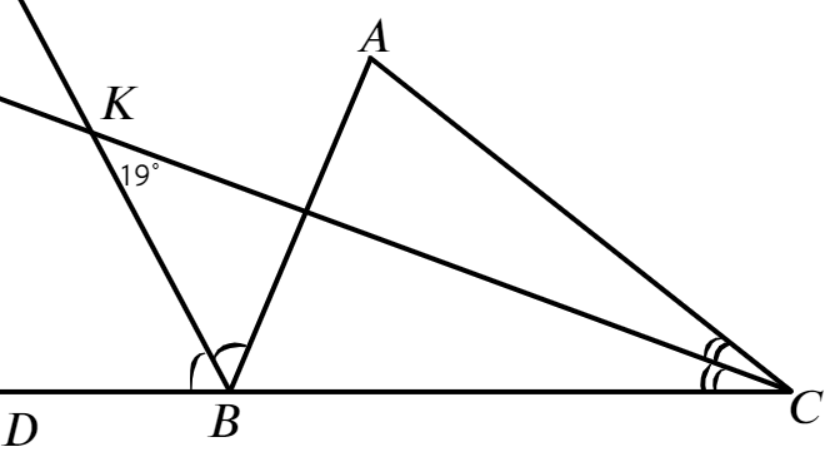
\includegraphics[scale=0.35]{g56.png}}
\end{figure}\\
Запишем сумму углов треугольника $BKC:\ 19^\circ+(180^\circ-\angle B):2+\angle B+\frac{1}{2}\angle C=180^\circ,\ \frac{1}{2}(\angle B+\angle C)=71^\circ,\ \angle B+\angle C=142^\circ.$ Тогда $\angle BAC=180^\circ-(\angle B+\angle C)=180^\circ-142^\circ=38^\circ.$
ewpage

oindent57. \begin{figure}[ht!]
\center{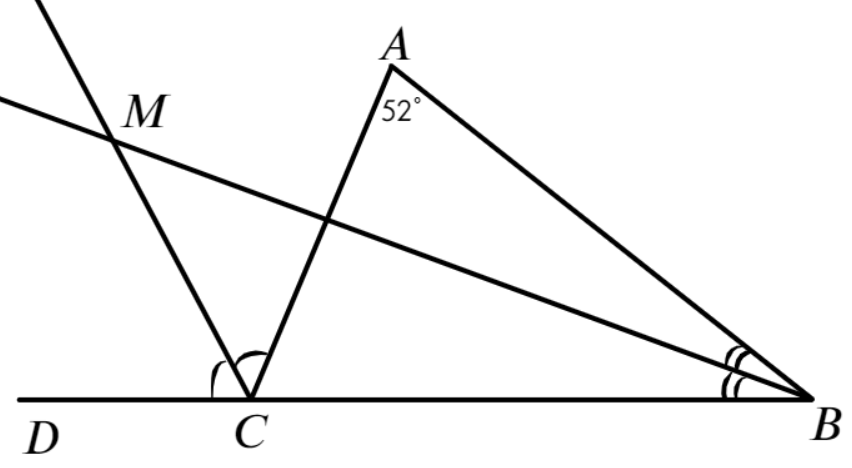
\includegraphics[scale=0.35]{g57.png}}
\end{figure}\\
Запишем сумму углов треугольника $ABC:\ \angle B+\angle C+52^\circ=180^\circ,\ \angle B+\angle C=128^\circ.$ Теперь запишем сумму углов треугольника $CMB:\ \angle BMC+(180^\circ-\angle C):2+\angle C+\frac{1}{2}\angle B=180^\circ,\ \angle BMC+\frac{1}{2}(\angle B+\angle C)=90^\circ,\ \angle BMC+64^\circ=90^\circ,\ \angle BMC=26^\circ.$\\
